% This is the Reed College LaTeX thesis template. Most of the work 
% for the document class was done by Sam Noble (SN), as well as this
% template. Later comments etc. by Ben Salzberg (BTS). Additional
% restructuring and APA support by Jess Youngberg (JY).
% Your comments and suggestions are more than welcome; please email
% them to cus@reed.edu
%
% See http://web.reed.edu/cis/help/latex.html for help. There are a 
% great bunch of help pages there, with notes on
% getting started, bibtex, etc. Go there and read it if you're not
% already familiar with LaTeX.
%
% Any line that starts with a percent symbol is a comment. 
% They won't show up in the document, and are useful for notes 
% to yourself and explaining commands. 
% Commenting also removes a line from the document; 
% very handy for troubleshooting problems. -BTS

% As far as I know, this follows the requirements laid out in 
% the 2002-2003 Senior Handbook. Ask a librarian to check the 
% document before binding. -SN

%%
%% Preamble
%%
% \documentclass{<something>} must begin each LaTeX document
\documentclass[12pt,twoside]{reedthesis}
% Packages are extensions to the basic LaTeX functions. Whatever you
% want to typeset, there is probably a package out there for it.
% Chemistry (chemtex), screenplays, you name it.
% Check out CTAN to see: http://www.ctan.org/
%%
\usepackage{graphicx,latexsym} 
\usepackage{amssymb,amsthm,amsmath}
\usepackage{longtable,booktabs,setspace} 
\usepackage{chemarr} %% Useful for one reaction arrow, useless if you're not a chem major
\usepackage[hyphens]{url}
\usepackage{rotating}
\usepackage{natbib}
\usepackage{ifthen}
\graphicspath{{./Figs/}} % Set graphics path
% Comment out the natbib line above and uncomment the following two lines to use the new 
% biblatex-chicago style, for Chicago A. Also make some changes at the end where the 
% bibliography is included. 
%\usepackage{biblatex-chicago}
%\bibliography{thesis}

% \usepackage{times} % other fonts are available like times, bookman, charter, palatino


%%%% REFERENCES %%%%%
\newcommand{\rf}     [1] {~\cite{#1}}
\newcommand{\refref} [1] {ref.~\cite{#1}}
\newcommand{\refRef} [1] {Ref.~\cite{#1}}
\newcommand{\refrefs}[1] {refs.~\cite{#1}}
\newcommand{\refRefs}[1] {Refs.~\cite{#1}}
\newcommand{\refeq}  [1] {(\ref{#1})}
\newcommand{\refeqs} [2]{(\ref{#1}--\ref{#2})}
\newcommand{\refex}  [1] {example~(\ref{#1})}
\newcommand{\refEx}  [1] {Example~(\ref{#1})}
\newcommand{\reffig} [1] {figure~\ref{#1}}
\newcommand{\reffigs} [2] {figures~\ref{#1} and~\ref{#2}}
\newcommand{\refFig} [1] {Figure~\ref{#1}}
\newcommand{\refFigs} [2] {Figures~\ref{#1} and~\ref{#2}}
\newcommand{\reftab} [1] {table~\ref{#1}}
\newcommand{\refTab} [1] {Table~\ref{#1}}
\newcommand{\reftabs}[2] {tables~\ref{#1} and~\ref{#2}}
\newcommand{\refsect}[1] {Section~\ref{#1}}
\newcommand{\refsects}[2] {Sections~\ref{#1} and \ref{#2}}
\newcommand{\refSect}[1] {Sect.~\ref{#1}}
\newcommand{\refSects}[2] {Sects.~\ref{#1} and \ref{#2}}
\newcommand{\refsecttosect}[2] {Sects.~\ref{#1} to~\ref{#2}}
\newcommand{\refappe}[1] {appendix~\ref{#1}}
\newcommand{\refappes}[2] {appendices~\ref{#1} and~\ref{#2}}
\newcommand{\refAppe}[1] {Appendix~\ref{#1}}
\newcommand{\refChapter}[1]{Chapter~\ref{#1}}
\newcommand{\refChapt}[1]{Chapt.~\ref{#1}}

%%%% SYMBOLS %%%%
\newcommand{\ReN}[1]{\ensuremath{Re}} % Reynolds number
\newcommand{\Hh}{\mathbb{H}}
\newcommand{\N}{\mathbb{N}}
\newcommand{\A}{\mathbb{A}}
\newcommand{\Z}{\mathbb{Z}}
\newcommand{\C}{\mathbb{C}}
\newcommand{\Q}{\mathbb{Q}}
\newcommand{\R}{\mathbb{R}}
\newcommand{\proj}{\mathbb{P}}
\newcommand{\G}{\mathbb{G}}

% homology commands
\newcommand{\K}{\mathcal{K}}
\newcommand{\Kd}{\K^{d}}
\newcommand{\emb}[1]{\mathord{\mr{emb}(#1)}}
\newcommand{\wh}[1]{\widehat{#1}}
\newcommand{\Qhat}{\wh{Q}}

\newcommand{\mr}{\mathrm}
\newcommand{\ith}{\textsuperscript{th}}

%%%% ABBREVIATIONS %%%%%
\newcommand{\etc}{{etc.}}       % APS
\newcommand{\etal}{{\em et al.}}    % etal in italics, APS too
\newcommand{\ie}{{i.e.}}        % APS
\newcommand{\cf}{{\em cf.\ }}     % APS
\newcommand{\eg}{{e.g.\ }}        % APS, OUP, hard space '\eg\ NextWord'

%%%%% ENVIRONMENTS %%%%%
\theoremstyle{plain}% default
\newtheorem{thm}{Theorem}[section]
\newtheorem{lem}[thm]{Lemma}
\newtheorem{prop}[thm]{Proposition}
\newtheorem*{cor}{Corollary}
\newtheorem*{KL}{Klein?s Lemma}

\theoremstyle{definition}
\newtheorem{defn}{Definition}[section]
\newtheorem{conj}{Conjecture}[section]
\newtheorem{exmp}{Example}[section]

\theoremstyle{remark}
\newtheorem*{rem}{Remark}
\newtheorem*{note}{Note}
\newtheorem{case}{Case}


%%%%% EDITING COMMANDS %%%%%
\newcommand{\DB}[2]{$\footnotemark\footnotetext{DB #1: {\color{red}#2}}$} %date, comment
\newcommand{\DBedit}[1]{{\color{red}#1}}
\newcommand{\JH}[2]{$\footnotemark\footnotetext{DB #1: {\color{red}#2}}$} %date, comment
\newcommand{\JHedit}[1]{{\color{red}#1}} % Load thesis specific macros

\title{My Final College Paper}
\author{Your R. Name}
% The month and year that you submit your FINAL draft TO THE LIBRARY (May or December)
\date{May 200x}
\division{Mathematics and Natural Sciences}
\advisor{Advisor F. Name}
%If you have two advisors for some reason, you can use the following
%\altadvisor{Your Other Advisor}
%%% Remember to use the correct department!
\department{Mathematics}
% if you're writing a thesis in an interdisciplinary major,
% uncomment the line below and change the text as appropriate.
% check the Senior Handbook if unsure.
%\thedivisionof{The Established Interdisciplinary Committee for}
% if you want the approval page to say "Approved for the Committee",
% uncomment the next line
%\approvedforthe{Committee}

\setlength{\parskip}{0pt}
%%
%% End Preamble
%%
%% The fun begins:
\begin{document}

  \maketitle
  \frontmatter % this stuff will be roman-numbered
  \pagestyle{empty} % this removes page numbers from the frontmatter

% Acknowledgements (Acceptable American spelling) are optional
% So are Acknowledgments (proper English spelling)
	% Acknowledgements (Acceptable American spelling) are optional
% So are Acknowledgments (proper English spelling)
    \chapter*{Acknowledgements}
    
It has only recently dawned on me what this process has meant to me. Post-ironic affectation aside, I genuinely love and appreciate everything that this school has done for me; how it has motivated me, inspired me academically and artistically, frustrated me, and pushed me to the end of my rope.

Of course, it is not the institution of Reed itself I have to thank. It is the individuals: my friends, my colleagues, and my mentors. I must first acknowledge my advisor Daniel for holding my hand through this entire exercise, guiding me through darkness when I felt like I was just hiding here. Next, I owe much of my growth as an artist to Marisa who never let my (many) opinions go unchallenged. I could not show enough gratitude towards my mother and father who have encouraged me in every endeavor. I must lastly thank Drew, Theo, and Monty. You have supported me when I've flailed, congratulated me in my successes, humored me in failure, and greatly shaped who I claim to be in this moment. Your close friendship has truly been the most meaningful aspect of my adult life; for that, I reserve a special place for the memories of our time at Reed.

% The preface is optional
% To remove it, comment it out or delete it.
	% The preface is optional
% To remove it, comment it out or delete it.
    \chapter*{Preface}
	This is an example of a thesis setup to use the reed thesis document class.

  \tableofcontents
% if you want a list of tables, optional
  \listoftables
% if you want a list of figures, also optional
  \listoffigures
		
% The abstract is not required if you're writing a creative thesis (but aren't they all?)
% If your abstract is longer than a page, there may be a formatting issue.
	% The abstract is not required if you're writing a creative thesis (but aren't they all?)
% If your abstract is longer than a page, there may be a formatting issue.
    \chapter*{Abstract}

A method of topological analysis known as computational homology is explored in the context of the Gray-Scott reaction-diffusion model. Using the homology information of patterns generated by simulations of Gray-Scott, namely the Betti numbers, the Shannon entropy $S$ is calculated over a large set of parameters to elucidate features about the system. The results of the calculation show strong qualitative agreement with previous nonlinear analysis of the Gray-Scott system. Other applications of homology theory and the problems encountered therein are also discussed.
	\newpage
\vspace*{0.33\textheight}
\begin{center}
\textit{For mom and dad.}
\end{center}

  \mainmatter % here the regular arabic numbering starts
  \pagestyle{fancyplain} % turns page numbering back on

% Double spacing: if you want to double space, or one and a half 
% space, uncomment one of the following lines. You can go back to 
% single spacing with the \singlespacing command.
% \onehalfspacing
% \doublespacing

	%The \introduction command is provided as a convenience.
%if you want special chapter formatting, you'll probably want to avoid using it altogether
		
\chapter*{Introduction}
    \addcontentsline{toc}{chapter}{Introduction}
		\chaptermark{Introduction}
		\markboth{Introduction}{Introduction}
% The three lines above are to make sure that the headers are right, that the intro gets included in the table of contents, and that it doesn't get numbered 1 so that chapter one is 1.
The study of pattern formation is incredibly diverse and certainly one of the most compelling aspects of nonlinear phenomenology. Scientists from many disciplines study pattern formation on scales ranging from that of the entire universe all the way down to the microscopic.\footnote{See the introduction of Cross \& Greenside for an overview of the study of pattern formation\rf{cross_greenside_2009}.} Just a cursory glance at the structure of a wind-swept sand dune, a snowflake, or even our own spiral galaxy reveals something interesting. Observation of these patterns might lead a scientist to ask what causes the pattern and wonder why there are patterns at all. This question gets complicated quickly because whether you see `God in the patterns' or see them as the result of a non-equilibrium universe, there is still the question of what it means to have ``structure'' or ``complexity'' or even to be ``interesting''.
%
\begin{figure}[h]
	\centering
	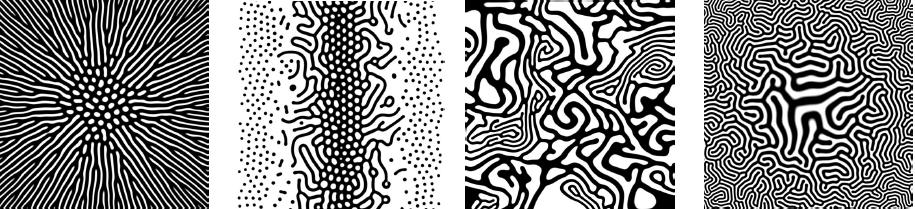
\includegraphics[width=\textwidth]{rd_examples.png}
	\caption{Patterns of the Gray-Scott reaction-diffusion system simulated by Karl Sims. Figure adapted from \protect\bibentry{karlsims}.}
	\label{fig:karl_sims}
\end{figure}

	Of course, patterns in nature are inherently difficult to understand; they are often inhomogeneous, subject to many unknown forces, or simply too large or small to study carefully. So before arriving at conclusions about the structure of the universe, it is helpful to look at idealized systems. This can mean a tightly controlled experimental setup\rf{kurtuldu_2011} or a completely computational model like the one discussed here; \refFig{fig:karl_sims} shows the patterns formed by simulations of the Gray-Scott chemical reaction-diffusion model\rf{karlsims}. Indeed, the vast amount of literature on the study of pattern formation looks to these simplified, yet no less dazzling, ``prepared patterns'' to draw conclusions about natural patterns\rf{cross_greenside_2009}. One heavily studied example is Rayleigh-B\'{e}nard convection, the experimental setup for which is extremely accessible; a horizontal plane of fluid is heated from below and cooled from above which gives rise to patterns like the one shown in \refFig{fig:rbconvec}.
%
\begin{figure}[h]
	\centering
	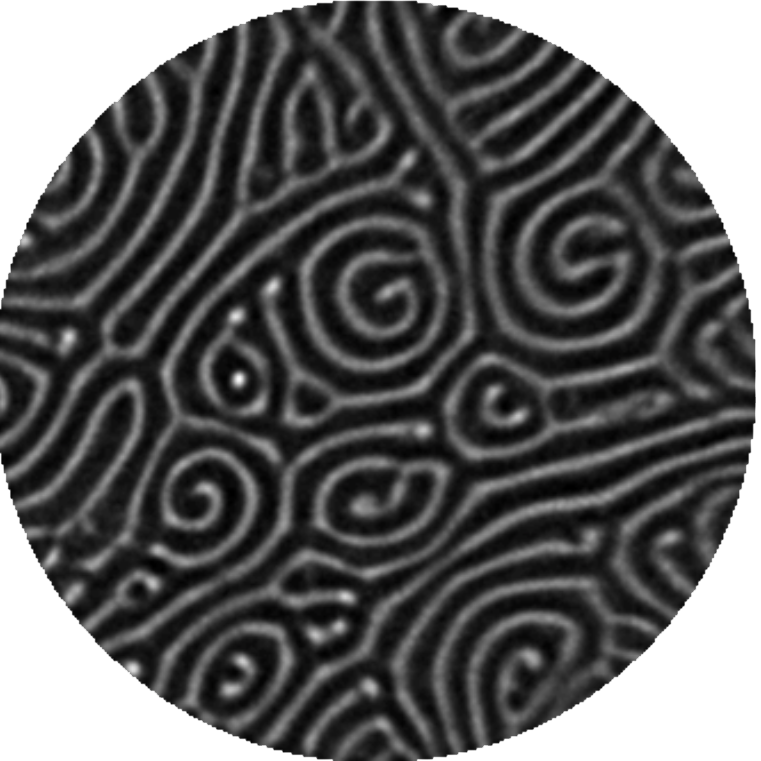
\includegraphics[width=0.3\textwidth]{rbconvec.png}
	\caption{An image of the ``prepared pattern'' formed by Rayleigh-B\'{e}nard convection. A horizontal plane of fluid is heated from below and cooled from above. Dark regions indicate the hot upflows and bright regions indicate cold downflows. Figure adapted from \protect\bibentry{kurtuldu_2011}.}
	\label{fig:rbconvec}
\end{figure}
%

	The study of patterns often comes down to the study of \textit{image data}, especially in the setting of a computational simulation. There are many mathematical tools available to help interpret this kind of data but as the complexity of our information (i.e.\ the amount of data) increases, it becomes increasingly difficult to parse relevant information.  Technological development in recent years not only makes capturing massive amounts of data possible, but commonplace. In the world of medical imaging, for example, data sets of X-Ray tomography, which allow for 3D reconstruction of biological structures such as the heart or lungs, can easily exceed dozens of gigabytes. While the increasing availability of data would serve only to improve our understanding of these systems, it is only as useful as our analytical methods allow. Traditional techniques may fall flat in the face of exceedingly sophisticated information.
	
\begin{figure}[h]
        \centering
        \begin{subfigure}[b]{0.35\textwidth}
        	\centering
                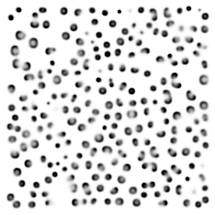
\includegraphics[width=0.85\textwidth]{alpha_v_grey.png}
                \caption{Pattern type $\alpha$.}
                \label{fig:alphagrey_fft}
        \end{subfigure}
        \begin{subfigure}[b]{0.35\textwidth}
        	\centering
                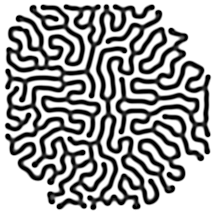
\includegraphics[width=0.85\textwidth]{kappa_v_grey.png}
                \caption{Pattern type $\kappa$.}
                \label{fig:kappagrey_fft}
        \end{subfigure} \\
        
        \begin{subfigure}[b]{0.35\textwidth}
        	\centering
                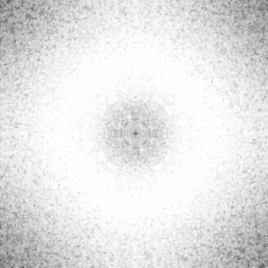
\includegraphics[width=0.85\textwidth]{alpha_v_fft.png}
                \caption{Fourier Transform of $\alpha$.}
                \label{fig:alphafft}
        \end{subfigure}
        \begin{subfigure}[b]{0.35\textwidth}
        	\centering
                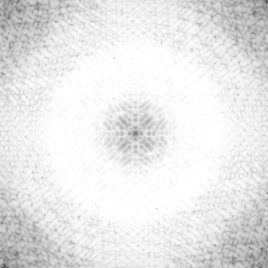
\includegraphics[width=0.85\textwidth]{kappa_v_fft.png}
                \caption{Fourier Transform of $\kappa$.}
                \label{fig:kappafft}
        \end{subfigure}
        \caption{Two very distinct pattern types of the Gray-Scott reaction-diffusion system, $\alpha$ and $\kappa$ (described further in \refsect{sect:gsmodel}). The Fourier transform of each pattern is hard to distinguish by eye and extracting meaningful information is difficult. The problematic nature of this method motivates our need for other, perhaps lower-level, analytic techniques.}\label{fig:fourierfail}
\end{figure}

	Take for example the Fourier transform, a powerful method for analysis which is often used to remove noise or apply filters to images. We would expect the Fourier transform to provide some insight into the spatial frequency of the image\footnote{In this case, the Fourier transform converts from the \textit{spatial domain}, the image we see, to the \textit{frequency domain}. The FT has been used for intricate pattern recognition, see\rf{hui_2014}.}, but in some cases, this method fails to provide useful information. Examine the two distinct pattern types of the Gray-Scott reaction-diffusion system shown in \refFig{fig:fourierfail} (more about this system in \refsect{sect:gsmodel}). The two pattern types $\alpha$ and $\kappa$ (\refFigs{fig:alphagrey_fft}{fig:kappagrey_fft} respectively) are easy to differentiate by eye yet the Fourier transforms (\refFigs{fig:alphafft}{fig:kappafft}) are disappointingly similar. Although this method is capable of extracting useful information, we would like some way to supplement our findings. The need for new methods arises and many times that means starting at the lowest level (\ie the structures that make up the image) especially when the crucial information is geometric in nature.
	
	But for many systems, it doesn't make sense to attempt to describe basic geometric structures in terms of the underlying mathematical equations (assuming we can write them down in the first place). This problem calls for a framework that gets at the geometric information even when face with numerical error and minor perturbations. The theory of computational homology described in \refChapter{ch:homology} does just this. Under the umbrella of algebraic topology, homology provides a beautiful framework for transforming topology into algebra from which one can draw insight into global properties. Although homology has only recently been brought to the fore of experimental physics, its application has shown interesting results\rf{kaczynski_2007,mischaikow_2002,gameiro_2004,mischaikow_2006}. This project explores the application of this theory to one pattern forming system in particular and highlights the information that may be derived from it.
	
	\chapter{Reaction-Diffusion Systems}

	Reaction-diffusion (RD) systems are models that determine how concentrations of chemical species change in space and time. These systems are driven by two processes: chemical reaction and spatial diffusion. RD systems are governed by partial differential equations, the most basic of which might look something like
	\begin{align}
		\frac{\partial u}{\partial t} = d \nabla^2 u + r(u).
		\label{eq:KPP}
	\end{align}

This is sometimes called the Kolmogorov-Petrovsky-Piskounov equation in which $u$ is a generic chemical species, $d$ is a diffusion coefficient, $\nabla^2 u$ is the Laplace operator, and $r(u)$ is a general reaction term. Of course, RD systems consisting of a single chemical do not form interesting patterns since there is no reaction taking place.

	RD systems are interesting because their solutions can show wide variety of complex patterns, many of which resemble patterns of nature such as spirals, stripes, and spots\rf{pearson_1993}. One drawback of the simplicity of these systems is that quantitative comparison to experimental systems is difficult. Alan Turing, one of the first to study RD systems in detail, acknowledged this in the famous opening lines of his 1952 paper\rf{turing_1952}:
%
\begin{quote}
In this section a mathematical model of the growing embryo will be described. This model will be a simplification and an idealization, and consequently a falsification. It is to be hoped that the features retained for discussion are those of greatest importance in the present state of knowledge.
\end{quote}
%
	Despite this concession, reaction-diffusion systems constitute an important part of the study of nonlinear dynamics today. Turing went on to suggest that reaction-diffusion systems of morphogens, chemicals that govern the pattern of embryo tissue development, may be able to explain the presence of spots or stripes on an organism. Although the science behind animal patterns is more complicated, Turing laid the framework by which patterns form from minor perturbations of otherwise homogenous systems. Since then, many others have noted the similarity between RD patterns and patterns in nature\rf{bard_1974,bard_1981,murray_1981,meinhardt_1982,young_1984,turk_1991,witkin_1991}. \refFig{fig:witkin} provides an example of how patterns formed by reaction-diffusion systems have been used to generate natural-looking textures in the context of computer graphics.

\begin{figure}[h]
	\centering
	\includegraphics[width=0.8\textwidth]{witkin}
         \caption{Patterns generated by reaction diffusion systems. Witkin compares these patterns to those of nature\rf{witkin_1991}; ``Row 1: reptile, giraffe, coral, scalloped. Row 2: spiral, triweave, twisty maze, replication, purple thing. Row 3: sand, maze, zebra haunch, radial. Row 4: space giraffe, zebra, stucco, beats us.'' Adapted from \protect\bibentry{witkin_1991}.} \label{fig:witkin}
\end{figure}
	
\section{The Gray-Scott model} \label{sect:gsmodel}
	One important model in the study of pattern formation is the Gray-Scott system which models the reaction of two generic chemical species, $U$ and $V$\rf{grayscott_1984}. The model is based on the chemical reaction
	\begin{align}
	\begin{split}
		U + 2V &\rightarrow 3V \\
		V &\rightarrow P,
		\label{eq:gs-chem}
	\end{split}
	\end{align}
where $V$ is converted to an inert product, $P$, which doesn't interfere with the reaction of the system. $V$ appears on both sides of the chemical reaction and thus catalyzes its own production. Gray and Scott developed the following set of non-dimensional partial differential equations (PDEs) in which $u$ and $v$ represent the concentrations of chemicals $U$ and $V$ respectively.
	\begin{align}
		\frac{\partial u}{\partial t} & = d_u \nabla^2 u - uv^2 + F(1-u) \label{eq:gsu} \\
		\frac{\partial v}{\partial t} & = d_v \nabla^2 v  + uv^2 - (F +k)v \label{eq:gsv}
	\end{align}
We see that both equations take the form of \refeq{eq:KPP} except $u$ and $v$ are coupled. The boundary conditions are periodic and for simplicity, $d_u$, $d_v$, $F$, and $k$ are taken to be constants. The first terms in each equation, $d_u \nabla^2 u$ and $d_v \nabla^2 v$, are the diffusion terms. The Laplace operator, $\nabla^2$, is responsible for the diffusion of each chemical in space (like the diffusion of heat in the more familiar heat equation) while the \textit{diffusion coefficients}, $d_u$ and $d_v$, govern the diffusion rate. The $\pm uv^2$ terms are the  \textit{reaction terms} which convert $U$ into $V$; an increase in $v$ is equal to the decrease in $u$, hence $+uv^2$ in \refeq{eq:gsv}. Since $U$ will eventually get used up to generate $V$, the term $F(1-u)$ is the \textit{replenishment term} which reintroduces chemical $U$ into the system ($u$ has a maximum value of 1). Similarly, chemical $V$ would increase without limit except for the \textit{diminishment term}, $(F+k)v$, which serves to remove chemical $V$ from the system. $F$ is referred to the \textit{feed rate} and determines the rate of replenishment while $k$ is the difference between this rate and that of chemical $V$.

For some biological intuition, one can imagine the chemical reactions that occur in the development of an embryo as Turing theorized. In this case, the supply of chemicals might be the bloodstream where the replenishment and diminishment rates of the reaction are determined by the permeability of cell membranes.

The Gray-Scott system is particularly notable for the wide range of irregular patterns it produces. Previous analysis of the system by Pearson\rf{pearson_1993} identified at least 12 different pattern types, all of which occur at different $F, k$ with $d_u = 2 d_v$.\footnote{Turing instabilities, which give rise to spontaneous pattern formation, cannot occur if all diffusion coefficients are equal. The ratio of 2 for diffusion coefficients has been found to show symmetry breaking for a wide range of parameter values\rf{pearson_1993}.} \refFig{fig:pearson} shows the 12 quantifiably different patterns observed in this system which Pearson classfied using standard methods of nonlinear analysis (\eg linear stability analysis and bifurcation theory)\rf{strogatz_2001}. The chemical concentration of $U$ is plotted over a $256 \times 256$ computational domain. The wide variety of observable patterns reveals the extremely variable behavior of this system as parameters are varied. \refFig{fig:fk_pspace} provides a legend for the patterns, mapping each of them to their locations in $k, F$ parameter space. One of the most compelling qualities of these patterns is their resemblance to patterns of nature. For example, $\kappa$ (\refFig{fig:kappa_sample}) looks like coral and $\lambda$ (\refFig{fig:lambda_sample}) resembles the growth of bacteria. Other patterns, like $\beta$ (\refFig{fig:beta_sample}), exhibit complex spatiotemporal behavior that resembles turbulence.

\begin{figure}
	\centering
	\begin{subfigure}[b]{0.2\textwidth}
                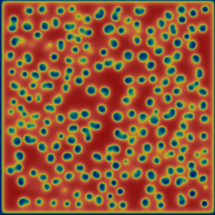
\includegraphics[width=\textwidth]{alpha_sample.png}
                \caption{$\alpha$}
                \label{fig:alpha_sample}
        \end{subfigure}%
        ~ %add desired spacing between images, e. g. ~, \quad, \qquad, \hfill etc.
          %(or a blank line to force the subfigure onto a new line)
        \begin{subfigure}[b]{0.2\textwidth}
                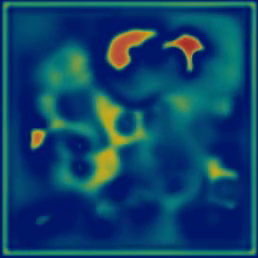
\includegraphics[width=\textwidth]{beta_sample.png}
                \caption{$\beta$}
                \label{fig:beta_sample}
        \end{subfigure}
        \begin{subfigure}[b]{0.2\textwidth}
                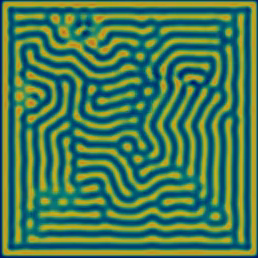
\includegraphics[width=\textwidth]{gamma_sample.png}
                \caption{$\gamma$}
                \label{fig:gamma_sample}
        \end{subfigure}
        \begin{subfigure}[b]{0.2\textwidth}
                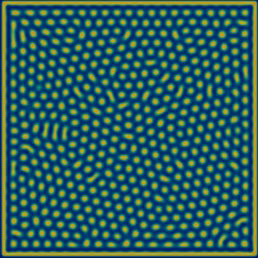
\includegraphics[width=\textwidth]{delta_sample.png}
                \caption{$\delta$}
                \label{fig:delta_sample}
        \end{subfigure} \hfill \\
         \begin{subfigure}[b]{0.2\textwidth}
                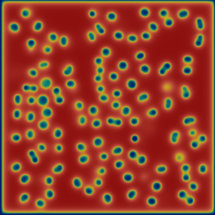
\includegraphics[width=\textwidth]{epsilon_sample.png}
                \caption{$\epsilon$}
                \label{fig:epsilon_sample}
        \end{subfigure}
        \begin{subfigure}[b]{0.2\textwidth}
                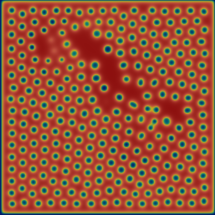
\includegraphics[width=\textwidth]{zeta_sample.png}
                \caption{$\zeta$}
                \label{fig:zeta_sample}
        \end{subfigure}
        \begin{subfigure}[b]{0.2\textwidth}
                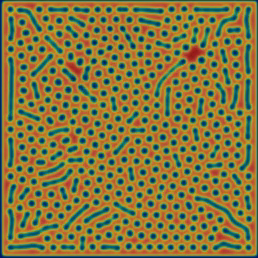
\includegraphics[width=\textwidth]{eta_sample.png}
                \caption{$\eta$}
                \label{fig:eta_sample}
        \end{subfigure}
        \begin{subfigure}[b]{0.2\textwidth}
                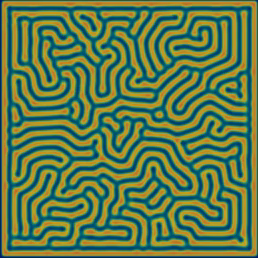
\includegraphics[width=\textwidth]{theta_sample.png}
                \caption{$\theta$}
                \label{fig:theta_sample}
        \end{subfigure} \hfill \\
        \begin{subfigure}[b]{0.2\textwidth}
                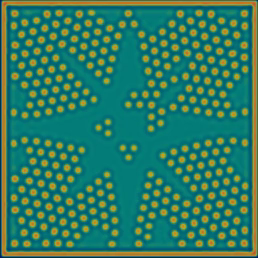
\includegraphics[width=\textwidth]{iota_sample.png}
                \caption{$\iota$}
                \label{fig:iota_sample}
        \end{subfigure}
         \begin{subfigure}[b]{0.2\textwidth}
                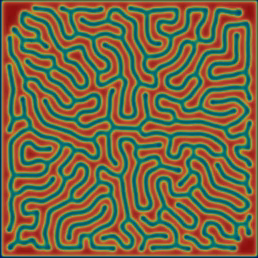
\includegraphics[width=\textwidth]{kappa_sample.png}
                \caption{$\kappa$}
                \label{fig:kappa_sample}
        \end{subfigure}
        \begin{subfigure}[b]{0.2\textwidth}
                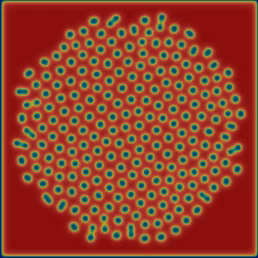
\includegraphics[width=\textwidth]{lambda_sample.png}
                \caption{$\lambda$}
                \label{fig:lambda_sample}
        \end{subfigure}
        \begin{subfigure}[b]{0.2\textwidth}
                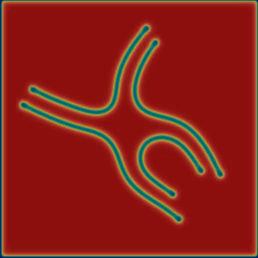
\includegraphics[width=\textwidth]{mu_sample.png}
                \caption{$\mu$}
                \label{fig:mu_sample}
        \end{subfigure} \hfill
        \caption{Patterns of chemical concentration $U$ identified in\rf{pearson_1993}. Each pattern, \refFig{fig:alpha_sample}---\refFig{fig:mu_sample}, is designated by a Greek letter which corresponds to the plot in \refFig{fig:fk_pspace}. Red and blue indicate $U=1$ and $U\approx 0.2$ respectively. Note that a concentration plot of chemical $V$ would appear as the inverse of $U$ with red and blue swapped. Video simulations of each of these pattern types are available online at \url{http://joelhawkins.info/thesis}.}\label{fig:pearson}
\end{figure}

\begin{figure}[h]
	\centering
	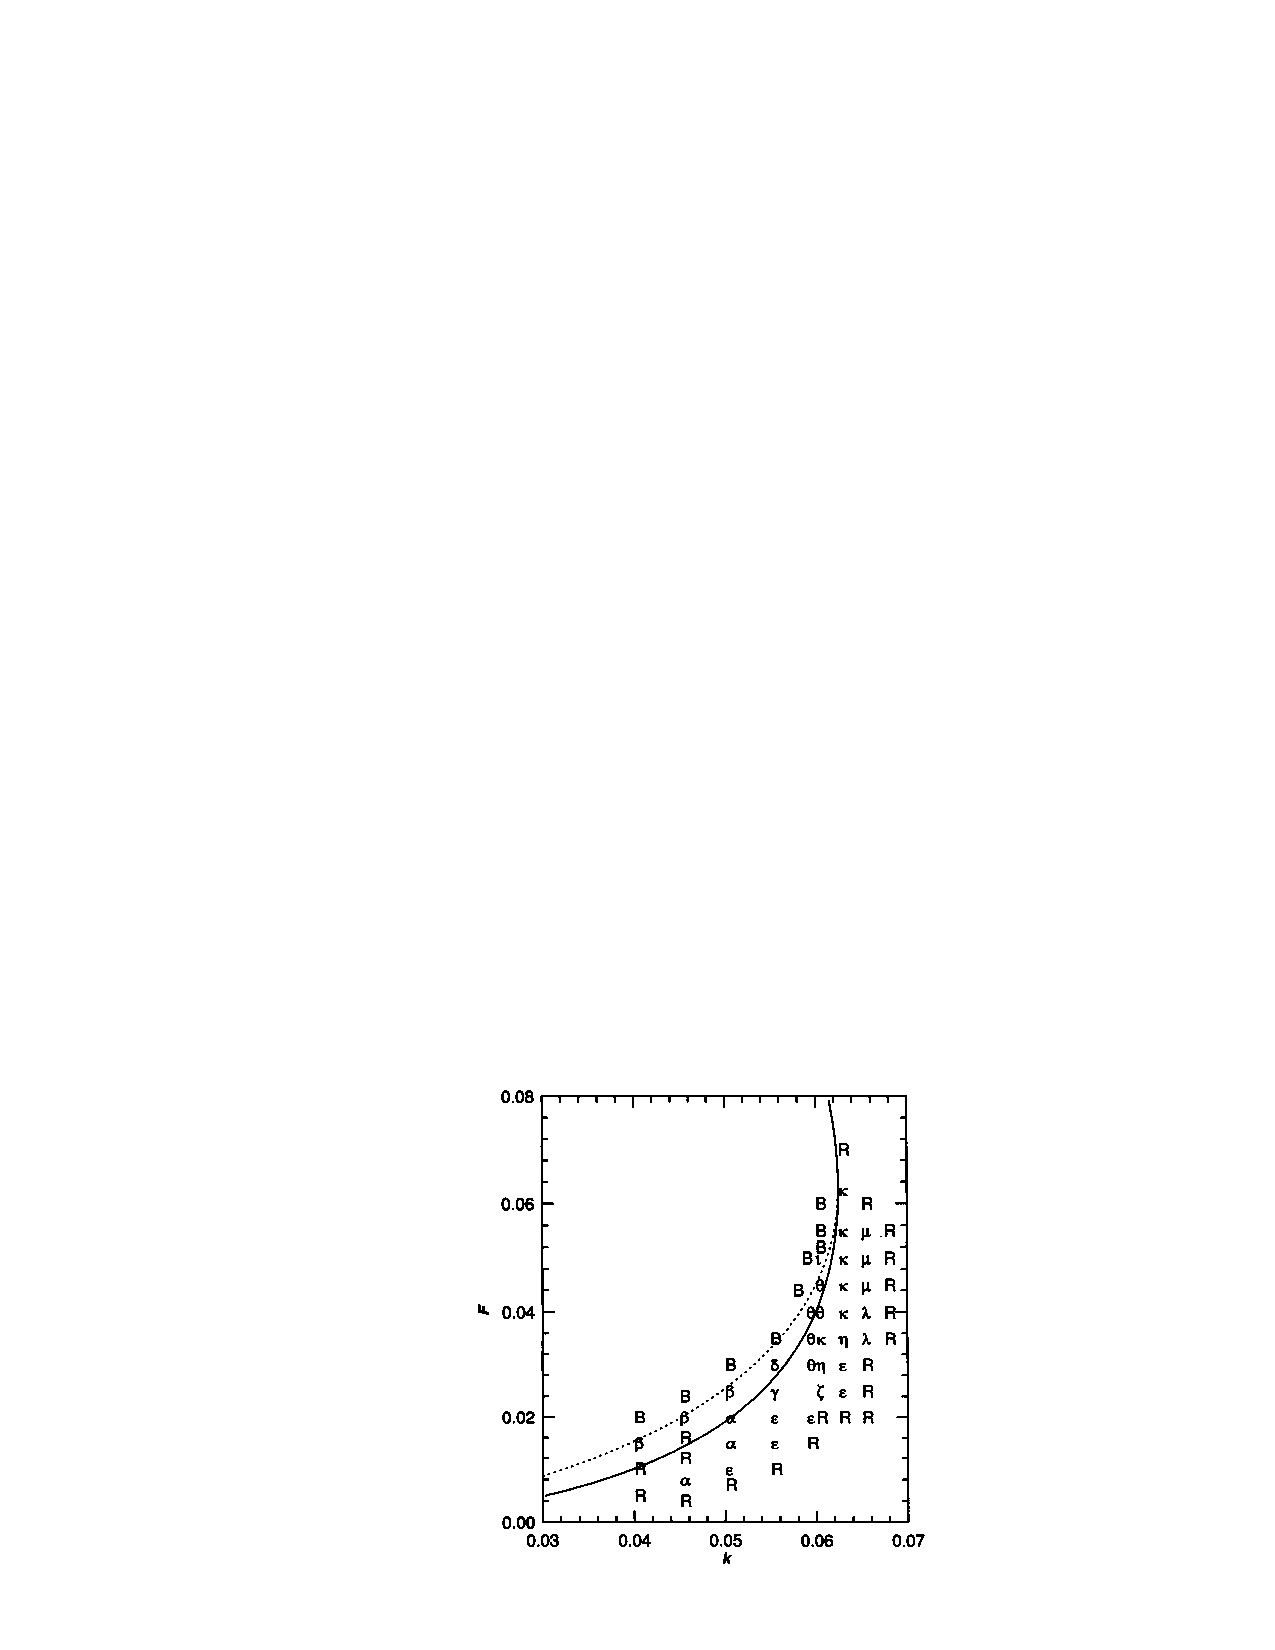
\includegraphics[width=0.5\columnwidth]{fk_pspace}
	\caption{The mapping of Greek letters in \refFig{fig:pearson} to their location in $k, F$ parameter space. R and B indicate that the system evolved to uniform red and blue states respectively. This figure also represents a phase diagram of the reaction kinetics. Between the solid and dotted line, the system is bistable for which there are two linearly stable steady states. As $f$ passes below the dotted line, the non-trivial steady state becomes unstable through Hopf bification giving stable periodic orbits for $k < 0.035$ and unstable ones for $k > 0.035$. The trivial state, ($U =1$, $V = 0$) exists for all $(f,k)$ outside the solid line. Adapted from \protect\bibentry{pearson_1993}.} \label{fig:fk_pspace}
\end{figure}

\section{Numerical simulation} \label{ch1:gs-simulation}

For the calculations described here, \refeqs{eq:gsu}{eq:gsv} are solved by forward Euler integration of the discrete Laplacian. This is obtained by the finite difference method and given by
	\begin{align}\label{eq:laplacian}
		\nabla^2 u(x,y) \approx u(x-1, y) + u(x+1, y) + u(x, y-1) + u(x, y+1) - 4 u(x, y),
	\end{align}
and similarly for $v$. In the Python programming language, this can be easily implemented using the Numpy package as below (see \refAppe{appB:gs-code} for full code).
%
\begin{Verbatim}[fontsize=\footnotesize,frame=leftline,framesep=5mm]
Lu = ( U[0:-2,1:-1] + U[2: ,1:-1] + 
       U[1:-1,0:-2] + U[1:-1,2: ] - 4*U[1:-1,1:-1] )  # Laplacian matrix for u
Lv = ( V[0:-2,1:-1] + V[2: ,1:-1] + 
       V[1:-1,0:-2] + V[1:-1,2: ] - 4*V[1:-1,1:-1] )  # Laplacian matrix for v

uvv = u*v*v    # corresponds to uv^2 term
u += (Du*Lu - uvv + F * (1-u)  ) # concentration matrix for u
v += (Dv*Lv + uvv - (F+k)*v    ) # concentration matrix for v
\end{Verbatim}
%
The matrices $u$ and $v$ contain concentration values for all points in the mesh. By iterating this calculation and plotting $u$ and $v$ as concentration maps, we can observe the evolution of the concentrations in time. The numerical accuracy of this solution is limited by the discretization of the Laplacian in \refeq{eq:laplacian} which is second-order accurate.

A spatial grid of $256 \times 256$ points constitutes the mesh with a time step of 1.\footnote{There are no qualitative differences for domain sizes up to $1024 \times 1024$ and time steps as low as $0.01$. Initial conditions also have little to no effect on the qualitative features of the resulting pattern after some time\rf{pearson_1993}.} The system was initialized with the state $U=1$, $V=0$ with a $40 \times 40$ area located symmetrically in the center perturbed with $U=0.5$, $V=0.25$. This square area is then further sprinkled with 1\% random ``noise'' to catalyze the reaction. The patterns in \refFig{fig:pearson} were generated using this method and depict the concentration of chemical $U$. A plot of chemical $V$ would appear as the inverse of $U$ so only $U$ is shown.

For each $F, k$, the simulation is run for 25,000 time steps. Every 10th image of the simulation is saved, so a total of 2,500 PNG files are produced to describe the time evolution of each pattern. The resulting images used for the analysis described in \refChapter{ch:methods} use a greyscale colormap like that of \refFig{fig:fourierfail}.





	\chapter{Mathematics and Science}	
\section{Math}
	\TeX\ is the best way to typeset mathematics. Donald Knuth designed \TeX\ when he got frustrated at how long it was taking the typesetters to finish his book, which contained a lot of mathematics. 
	
	If you are doing a thesis that will involve lots of math, you will want to read the following section which has been commented out. If you're not going to use math, skip over this next big red section. (It's red in the .tex file but does not show up in the .pdf.)
	
% MATH and PHYSICS majors: Uncomment the following section	
	$$\sum_{j=1}^n (\delta\theta_j)^2 \leq {\frac{\beta_i^2}{\delta_i^2 + \rho_i^2}}
\left[ 2\rho_i^2 + \frac{\delta_i^2\beta_i^2}{\delta_i^2 + \rho_i^2} \right] \equiv \omega_i^2
$$

From Informational Dynamics, we have the following (Dave Braden):

After {\it n} such encounters the posterior density for $\theta$ is

$$
\pi(\theta|X_1< y_1,\dots,X_n<y_n) \varpropto \pi(\theta) \prod_{i=1}^n\int_{-\infty}^{y_i}
   \exp\left(-\frac{(x-\theta)^2}{2\sigma^2}\right)\ dx
$$



Another equation:

$$\det\left|\,\begin{matrix}%
c_0&c_1\hfill&c_2\hfill&\ldots&c_n\hfill\cr
c_1&c_2\hfill&c_3\hfill&\ldots&c_{n+1}\hfill\cr
c_2&c_3\hfill&c_4\hfill&\ldots&c_{n+2}\hfill\cr
\,\vdots\hfill&\,\vdots\hfill&
  \,\vdots\hfill&&\,\vdots\hfill\cr
c_n&c_{n+1}\hfill&c_{n+2}\hfill&\ldots&c_{2n}\hfill\cr
\end{matrix}\right|>0$$


Lapidus and Pindar, Numerical Solution of Partial Differential Equations in Science and
Engineering.  Page 54

$$
\int_t\left\{\sum_{j=1}^3 T_j \left(\frac{d\phi_j}{dt}+k\phi_j\right)-kT_e\right\}w_i(t)\ dt=0,
   \qquad\quad i=1,2,3. 
$$

L\&P  Galerkin method weighting functions.  Page 55

$$
\sum_{j=1}^3 T_j\int_0^1\left\{\frac{d\phi_j}{dt} + k\phi_j\right\} \phi_i\ dt 
   = \int_{0}^1k\,T_e\phi_idt, \qquad i=1,2,3 $$
   
Another L\&P (p145)

$$
\int_{-1}^1\!\int_{-1}^1\!\int_{-1}^1 f\big(\xi,\eta,\zeta\big) 
   = \sum_{k=1}^n\sum_{j=1}^n\sum_{i=1}^n w_i w_j w_k f\big( \xi,\eta,\zeta\big).
$$

Another L\&P (p126)

$$
\int_{A_e} (\,\cdot\,) dx dy = \int_{-1}^1\!\int_{-1}^1 (\,\cdot\,) \det[J] d\xi d\eta.
$$

\section{Chemistry 101: Symbols}
Chemical formulas will look best if they are not italicized. Get around math mode's automatic italicizing by using the argument \verb=$\mathrm{formula here}$=, with your formula inside the curly brackets.

So, $\mathrm{Fe_2^{2+}Cr_2O_4}$ is written \verb=$\mathrm{Fe_2^{2+}Cr_2O_4}$=\\
Exponent or Superscript: O$^{-}$\\
Subscript: CH$_{4}$\\

To stack numbers or letters as in $\mathrm{Fe_2^{2+}}$, the subscript is defined first, and then the superscript is defined.\\
Angstrom: {\AA}\\
Bullet: CuCl $\bullet$ 7H${_2}$O\\
Double Dagger: \ddag \/\\
Delta: $\Delta$\\
Reaction Arrows: $\longrightarrow$ or  $\xrightarrow{solution}$\\
Resonance Arrows: $\leftrightarrow$\\
Reversible Reaction Arrows: $\rightleftharpoons$ or $\xrightleftharpoons[ ]{solution}$ (the latter requires the chemarr package)\\


\subsection{Typesetting reactions}
You may wish to put your reaction in a figure environment, which means that LaTeX will place the reaction where it fits and you can have a figure legend if desired:
\begin{figure}[htbp]
\begin{center}
$\mathrm{C_6H_{12}O_6  + 6O_2} \longrightarrow \mathrm{6CO_2 + 6H_2O}$
\caption{Combustion of glucose}
\label{combustion of glucose}
\end{center}
\end{figure}

\subsection{Other examples of reactions}
$\mathrm{NH_4Cl_{(s)}} \rightleftharpoons \mathrm{NH_{3(g)}+HCl_{(g)}}$\\
$\mathrm{MeCH_2Br + Mg} \xrightarrow[below]{above} \mathrm{MeCH_2\bullet Mg \bullet Br}$

\section{Physics}

Many of the symbols you will need can be found on the math page (\url{http://web.reed.edu/cis/help/latex/math.html}) and the Comprehensive \LaTeX\ Symbol Guide (enclosed in this template download).  You may wish to create custom commands for commonly used symbols, phrases or equations, as described in Chapter \ref{commands}.

\section{Biology}
You will probably find the resources at \url{http://www.lecb.ncifcrf.gov/~toms/latex.html} helpful, particularly the links to bsts for various journals. You may also be interested in TeXShade for nucleotide typesetting (\url{http://homepages.uni-tuebingen.de/beitz/txe.html}).  Be sure to read the proceeding chapter on graphics and tables, and remember that the thesis template has versions of Ecology and Science bsts which support webpage citation formats. 

	\chapter{Tables and Graphics}

\section{Tables}
	The following section contains examples of tables, most of which have been commented out for brevity. (They will show up in the .tex document in red, but not at all in the .pdf). For more help in constructing a table (or anything else in this document), please see the LaTeX pages on the CUS site. 

\begin{table}[htdp] % begins the table floating environment. This enables LaTeX to fit the table where it works best and lets you add a caption.
\caption[Basic Table 1]{A Basic Table: Correlation of Factors between Parents and Child, Showing Inheritance} 
% The words in square brackets of the caption command end up in the Table of Tables. The words in curly braces are the caption directly over the table.
\begin{center} 
% makes the table centered
\begin{tabular}{c c c c} 
% the tabular environment is used to make the table itself. The {c c c c} specify that the table will have four columns and they will all be center-aligned. You can make the cell contents left aligned by replacing the Cs with Ls or right aligned by using Rs instead. Add more letters for more columns, and pipes (the vertical line above the backslash) for vertical lines. Another useful type of column is the p{width} column, which forces text to wrap within whatever width you specify e.g. p{1in}. Text will wrap badly in narrow columns though, so beware.
\toprule % a horizontal line, slightly thicker than \hline, depends on the booktabs package
  Factors &  Correlation between Parents \& Child & Inherited \\ % the first row of the table. Separate columns with ampersands and end the line with two backslashes. An environment begun in one cell will not carry over to adjacent rows.
  \midrule % another horizontal line
Education & -0.49 & Yes \\ % another row
Socio-Economic Status & 0.28 & Slight \\
Income & 0.08 & No\\
Family Size & 0.19 & Slight \\
Occupational Prestige &0.21 & Slight \\
\bottomrule % yet another horizontal line
\end{tabular}
\end{center}
\label{inheritance} % labels are useful when you have more than one table or figure in your document. See our online documentation for more on this.
\end{table}

	\clearpage 
%% \clearpage ends the page, and also dumps out all floats. 
%% Floats are things like tables and figures.

If you want to make a table that is longer than a page, you will want to use the longtable environment. Uncomment the table below to see an example, or see our online documentation.

	\begin{longtable}{||c|c|c|c||}
	 	\caption[Long Table]{An example of a long table, with headers that repeat on each subsequent page: Results from the summers of 1998 and 1999 work at Reed College done
by Grace Brannigan, Robert Holiday and Lien Ngo in 1998 and Kate Brown and
Christina Inman in 1999.}\\ \hline
	    	  \multicolumn{4}{||c||}{Chromium Hexacarbonyl} \\\hline
		   State & Laser wavelength & Buffer gas & Ratio of $\frac{\textrm{Intensity
at vapor pressure}}{\textrm{Intensity at 240 Torr}}$ \\ \hline
		  \endfirsthead
		\hline     State & Laser wavelength & Buffer gas & Ratio of
$\frac{\textrm{Intensity at vapor pressure}}{\textrm{Intensity at 240 Torr}}$\\
\hline
		    \endhead

	    $z^{7}P^{\circ}_{4}$ & 266 nm & Argon & 1.5 \\\hline
	    $z^{7}P^{\circ}_{2}$ & 355 nm & Argon & 0.57 \\\hline
	    $y^{7}P^{\circ}_{3}$ & 266 nm & Argon & 1 \\\hline
	    $y^{7}P^{\circ}_{3}$ & 355 nm & Argon & 0.14 \\\hline
	    $y^{7}P^{\circ}_{2}$ & 355 nm & Argon & 0.14 \\\hline
	    $z^{5}P^{\circ}_{3}$ & 266 nm & Argon & 1.2 \\\hline
	    $z^{5}P^{\circ}_{3}$ & 355 nm & Argon & 0.04 \\\hline
	    $z^{5}P^{\circ}_{3}$ & 355 nm & Helium & 0.02 \\\hline
	    $z^{5}P^{\circ}_{2}$ & 355 nm & Argon & 0.07 \\\hline
	    $z^{5}P^{\circ}_{1}$ & 355 nm & Argon & 0.05 \\\hline
	    $y^{5}P^{\circ}_{3}$ & 355 nm & Argon & 0.05, 0.4 \\\hline
	    $y^{5}P^{\circ}_{3}$ & 355 nm & Helium & 0.25 \\\hline
	    $z^{5}F^{\circ}_{4}$ & 266 nm & Argon & 1.4 \\\hline
	    $z^{5}F^{\circ}_{4}$ & 355 nm & Argon & 0.29 \\\hline
	    $z^{5}F^{\circ}_{4}$ & 355 nm & Helium & 1.02 \\\hline
	    $z^{5}D^{\circ}_{4}$ & 355 nm & Argon & 0.3 \\\hline
	    $z^{5}D^{\circ}_{4}$ & 355 nm & Helium & 0.65 \\\hline
	    $y^{5}H^{\circ}_{7}$ & 266 nm & Argon & 0.17 \\\hline
	    $y^{5}H^{\circ}_{7}$ & 355 nm & Argon & 0.13 \\\hline
	    $y^{5}H^{\circ}_{7}$ & 355 nm & Helium & 0.11 \\\hline
	    $a^{5}D_{3}$ & 266 nm & Argon & 0.71 \\\hline
	    $a^{5}D_{2}$ & 266 nm & Argon & 0.77 \\\hline
	    $a^{5}D_{2}$ & 355 nm & Argon & 0.63 \\\hline
	    $a^{3}D_{3}$ & 355 nm & Argon & 0.05 \\\hline
	    $a^{5}S_{2}$ & 266 nm & Argon & 2 \\\hline
	    $a^{5}S_{2}$ & 355 nm & Argon & 1.5 \\\hline
	    $a^{5}G_{6}$ & 355 nm & Argon & 0.91 \\\hline
	    $a^{3}G_{4}$ & 355 nm & Argon & 0.08 \\\hline
	    $e^{7}D_{5}$ & 355 nm & Helium & 3.5 \\\hline
	    $e^{7}D_{3}$ & 355 nm & Helium & 3 \\\hline
	    $f^{7}D_{5}$ & 355 nm & Helium & 0.25 \\\hline
	    $f^{7}D_{5}$ & 355 nm & Argon & 0.25 \\\hline
	    $f^{7}D_{4}$ & 355 nm & Argon & 0.2 \\\hline
	    $f^{7}D_{4}$ & 355 nm & Helium & 0.3 \\\hline
	    \multicolumn{4}{||c||}{Propyl-ACT} \\\hline
%	    State & Laser wavelength & Buffer gas & Ratio of $\frac{\textrm{Intensity
%at vapor pressure}}{\textrm{Intensity at 240 Torr}}$\\ \hline
	    $z^{7}P^{\circ}_{4}$ & 355 nm & Argon & 1.5 \\\hline
	    $z^{7}P^{\circ}_{3}$ & 355 nm & Argon & 1.5 \\\hline
	    $z^{7}P^{\circ}_{2}$ & 355 nm & Argon & 1.25 \\\hline
	    $z^{7}F^{\circ}_{5}$ & 355 nm & Argon & 2.85 \\\hline
	    $y^{7}P^{\circ}_{4}$ & 355 nm & Argon & 0.07 \\\hline
	    $y^{7}P^{\circ}_{3}$ & 355 nm & Argon & 0.06 \\\hline
	    $z^{5}P^{\circ}_{3}$ & 355 nm & Argon & 0.12 \\\hline
	    $z^{5}P^{\circ}_{2}$ & 355 nm & Argon & 0.13 \\\hline
	    $z^{5}P^{\circ}_{1}$ & 355 nm & Argon & 0.14 \\\hline
	    \multicolumn{4}{||c||}{Methyl-ACT} \\\hline
%	    State & Laser wavelength & Buffer gas & Ratio of $\frac{\textrm{Intensity
% at vapor pressure}}{\textrm{Intensity at 240 Torr}}$\\ \hline
	    $z^{7}P^{\circ}_{4}$ & 355 nm & Argon & 1.6, 2.5 \\\hline
	    $z^{7}P^{\circ}_{4}$ & 355 nm & Helium & 3 \\\hline
	    $z^{7}P^{\circ}_{4}$ & 266 nm & Argon & 1.33 \\\hline
	    $z^{7}P^{\circ}_{3}$ & 355 nm & Argon & 1.5 \\\hline
	    $z^{7}P^{\circ}_{2}$ & 355 nm & Argon & 1.25, 1.3 \\\hline
	    $z^{7}F^{\circ}_{5}$ & 355 nm & Argon & 3 \\\hline
	    $y^{7}P^{\circ}_{4}$ & 355 nm & Argon & 0.07, 0.08 \\\hline
	    $y^{7}P^{\circ}_{4}$ & 355 nm & Helium & 0.2 \\\hline
	    $y^{7}P^{\circ}_{3}$ & 266 nm & Argon & 1.22 \\\hline
	    $y^{7}P^{\circ}_{3}$ & 355 nm & Argon & 0.08 \\\hline
	    $y^{7}P^{\circ}_{2}$ & 355 nm & Argon & 0.1 \\\hline
	    $z^{5}P^{\circ}_{3}$ & 266 nm & Argon & 0.67 \\\hline
	    $z^{5}P^{\circ}_{3}$ & 355 nm & Argon & 0.08, 0.17 \\\hline
	    $z^{5}P^{\circ}_{3}$ & 355 nm & Helium & 0.12 \\\hline
	    $z^{5}P^{\circ}_{2}$ & 355 nm & Argon & 0.13 \\\hline
	    $z^{5}P^{\circ}_{1}$ & 355 nm & Argon & 0.09 \\\hline
	    $y^{5}H^{\circ}_{7}$ & 355 nm & Argon & 0.06, 0.05 \\\hline
	    $a^{5}D_{3}$ & 266 nm & Argon & 2.5 \\\hline
	    $a^{5}D_{2}$ & 266 nm & Argon & 1.9 \\\hline
	    $a^{5}D_{2}$ & 355 nm & Argon & 1.17 \\\hline
	    $a^{5}S_{2}$ & 266 nm & Argon & 2.3 \\\hline
	    $a^{5}S_{2}$ & 355 nm & Argon & 1.11 \\\hline
	    $a^{5}G_{6}$ & 355 nm & Argon & 1.6 \\\hline
	    $e^{7}D_{5}$ & 355 nm & Argon & 1 \\\hline

		\end{longtable}

   
   \section{Figures}
   
	If your thesis has a lot of figures, \LaTeX\ might behave better for you than that other word processor.  One thing that may be annoying is the way it handles ``floats'' like tables and figures. \LaTeX\ will try to find the best place to put your object based on the text around it and until you're really, truly done writing you should just leave it where it lies.   There are some optional arguments to the figure and table environments to specify where you want it to appear; see the comments in the first figure.

	If you need a graphic or tabular material to be part of the text, you can just put it inline. If you need it to appear in the list of figures or tables, it should be placed in the floating environment. 
	
	To get a figure from StatView, JMP, SPSS or other statistics program into a figure, you can print to pdf or save the image as a jpg or png. Precisely how you will do this depends on the program: you may need to copy-paste figures into Photoshop or other graphic program, then save in the appropriate format.
	
	Below we have put a few examples of figures. For more help using graphics and the float environment, see our online documentation.
	
	And this is how you add a figure with a graphic:
	\begin{figure}[h]
	% the options are h = here, t = top, b = bottom, p = page of figures.
	% you can add an exclamation mark to make it try harder, and multiple
	% options if you have an order of preference, e.g.
	% \begin{figure}[h!tbp]
	   
	       \centering
	    % DO NOT ADD A FILENAME EXTENSION TO THE GRAPHIC FILE
	    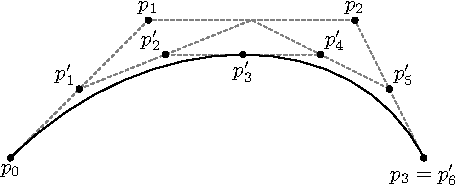
\includegraphics{subdivision}
	     \caption{A Figure}
	 \label{subd}
	\end{figure}

\clearpage %% starts a new page and stops trying to place floats such as tables and figures

\section{More Figure Stuff}
You can also scale and rotate figures.
 	\begin{figure}[h!]
	   
	       \centering
	    % DO NOT ADD A FILENAME EXTENSION TO THE GRAPHIC FILE
	    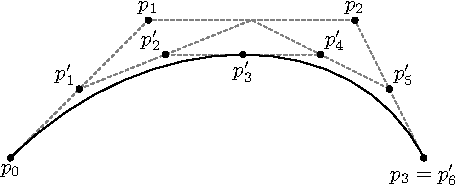
\includegraphics[scale=0.5,angle=180]{subdivision}
	    % if your figure shows up not where you want it, it may just be too big to fit. You can use the scale argument to shrink it, e.g. scale=0.85 is 85 percent of the original size. 
	     \caption{A Smaller Figure, Flipped Upside Down}
	 \label{subd2}
	\end{figure}

\section{Even More Figure Stuff}
With some clever work you can crop a figure, which is handy if (for instance) your EPS or PDF is a little graphic on a whole sheet of paper. The viewport arguments are the lower-left and upper-right coordinates for the area you want to crop.

 	\begin{figure}[h!]
	    	       \centering
	    % DO NOT ADD A FILENAME EXTENSION TO THE GRAPHIC FILE
	   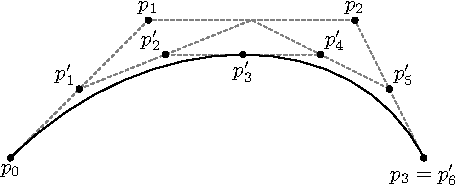
\includegraphics[clip=true, viewport=.0in .0in 1in 1in]{subdivision}
	    \caption{A Cropped Figure}
	 \label{subd3}
	\end{figure}
	
      \subsection{Common Modifications}
      The following figure features the more popular changes thesis students want to their figures. This information is also on the web at \url{web.reed.edu/cis/help/latex/graphics.html}.
           \renewcommand{\thefigure}{0.\arabic{figure}} %Renumbers the figure to the type 0.x
    \addtocounter{figure}{4} %starts the figure numbering at 4
    \begin{figure}[htbp]
    \begin{center}
   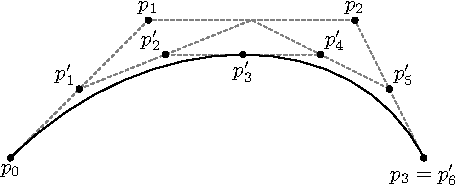
\includegraphics[scale=0.5]{subdivision}
    \caption[Flower type and percent specialization]{\footnotesize{Interaction bar plot showing the degree of specialization for each flower type.}} %the special ToC caption is in square brackets. The \footnotesize makes the figure caption smaller
    \label{barplot}
    \end{center}
    \end{figure} 

	\chapter*{Conclusion}
         \addcontentsline{toc}{chapter}{Conclusion}
	\chaptermark{Conclusion}
	\markboth{Conclusion}{Conclusion}
	\setcounter{chapter}{4}
	\setcounter{section}{0}
	
Throughout this thesis, we have tread the territory of nonlinear dynamics, computation, topology, and combinatorics. We have shown how the combination of these theories can produce novel and compelling results when presented with complex information. By examining patterns at their lowest level, looking closely at the fundamental geometric structures that make up the dazzling images we see, we can extract meaningful information and elucidate their properties. In this case, the analysis of the Gray-Scott system led us to calculate the entropy of the system over a wide range of parameters which both complements and confirms the analysis derived directly from the physics of the system.

The homology theory presented here has given us interesting insight into the dynamics of at least one pattern-forming model, but as I have endeavored to show, one can extend these techniques to \textit{any} topological object. This may be a single image, a video of an experiment, or a 4D construction of medical imaging data; the tools of homology are amazingly resilient and as computational methods evolve, these techniques may take precedence in the field of image analysis.

Of course, the findings in this thesis point towards many more avenues for further investigation of homology. One of the major problems confronted in this thesis is finding an appropriate threshold for which to perform the Betti number calculations. This could be solved with the implementation of an adaptive thresholding algorithm or, with a large leap in complexity, applying persistent homology (a relatively young theory at this time). Another interesting extension would be to use the time series information to derive more telling mathematical quantities such as the Lyapunov exponent which would confirm the chaotic dynamics of a system. It is certain that the applications of homology theory have not yet been exhausted; one of the virtues is that homology is so fundamental, its applications are wide open. It is my hope that the reader is convinced of its usefulness in the wake of increasingly complex data.

%If you feel it necessary to include an appendix, it goes here.
	\appendix

	\chapter{The First Appendix}

\section{Extra definitions, theorems, \etc}

\begin{defn} \label{ap:abeliandef}
	The \textit{free abelian group generated by a finite set}
	$$ S = \left\{s_1, s_2, \ldots, s_n \right\} $$
	is the set of all functions $ f : S \rightarrow \Z$, with the pointwise addition
		$$ (f + g)(s_i) := f(s_i) + g(s_i), \quad i = 1, 2, \ldots, n . $$
\end{defn}

\begin{defn} \label{ap:freeabeliandef}
	The \textit{free abelian group generated by a possibly infinite set} $S$ is the subgroup of $\Z^S$, consisting of all functions $f : S \rightarrow Z$ satisfying
	$$ f(s) = 0 \quad \text{for all but finitely many } s \in S. $$
\end{defn}
	\chapter{Code}

\section{Gray-Scott simulation code} \label{appB:gs-code}

The following code is written in the Python language. It requires the Numpy package which allows for easy and intuitive manipulation of matrices as well as Matplotlib to display the simulation. The procedure \textsc{runGS} takes four arguments: $d_u$, $d_v$, $F$, and $k$. By default, the domain size $n$ is set to 256.

\begin{Verbatim}[fontsize=\footnotesize,frame=leftline,framesep=5mm]
import numpy as np
import matplotlib.pyplot as plt

def runGS(Du, Dv, F, k):
  n = 256
  
  # create a structured n+2 by n+2 array of double precision floats
  Z = np.zeros((n+2,n+2), [('U', np.double), ('V', np.double)])
  U,V = Z['U'], Z['V']
  
  # u, v represent the concentrations of U, V
  u,v = U[1:-1,1:-1], V[1:-1,1:-1]
  
  # set initial conditions
  r = 20
  u[...] = 1.0  # set all u to 1.0
  U[n/2-r:n/2+r,n/2-r:n/2+r] = 0.50
  V[n/2-r:n/2+r,n/2-r:n/2+r] = 0.25
  
  # 'sprinkling' of random noise
  u += 0.05*np.random.random((n,n))
  v += 0.05*np.random.random((n,n))

  # set up plot
  plt.ion()

  # plot options
  size = np.array(Z.shape)
  dpi = 120.0
  figsize= size[1]/float(dpi),size[0]/float(dpi)
  fig = plt.figure(figsize=figsize, dpi=dpi, facecolor="white")
  fig.add_axes([0.0, 0.0, 1.0, 1.0], frameon=False)
  cmap = plt.cm.binary  # this is a greyscale colormap
  im = plt.imshow(V, interpolation='bicubic', cmap=cmap)  # show V in the plot
  plt.xticks([]), plt.yticks([])	

  # run simulation for 25000 time steps
  for i in xrange(25000):
    # discretized Laplacian matrix for u
    Lu = ( U[0:-2,1:-1] + U[2: ,1:-1] + 
       U[1:-1,0:-2] + U[1:-1,2: ] - 4*U[1:-1,1:-1] )
       
    # discretized Laplacian matrix for v
    Lv = ( V[0:-2,1:-1] + V[2: ,1:-1] + 
       V[1:-1,0:-2] + V[1:-1,2: ] - 4*V[1:-1,1:-1] )

    uvv = u*v*v  # the nonlinear term uv^2
      
    # change the concentrations in place
    u += (Du*Lu - uvv +  F   *(1-u))
    v += (Dv*Lv + uvv - (F+k)*v    )

    if i % 10 == 0:  # show only every 10 steps on the plot
      im.set_data(V)
      im.set_clim(vmin=0.0, vmax=0.4)  # set color limits
      plt.draw()
      # to save each figure
      plt.savefig('./gs/gs-%04d.png' % (i/10) ,dpi=dpi)

  plt.ioff()
  plt.close()
\end{Verbatim}

\section{Entropy calculation code}

The code below is used to calculate the entropy maps shown in \refFigs{fig:V144_fk_rs_entropy}{fig:UV_entropy_trans}. It is also written in the Python language and relies on a few extra packages. The procedure \textsc{bettiList} by examining a pairs of Betti numbers contained in a CSV file with rows of the form \texttt{time-step,b0,b1} where \texttt{b0,b1} indicate $\beta_0$ and $\beta_1$. \textsc{makeP\_i} uses this list to count the number of times each pair \verb+{b0,b1}+ (interpreted simply as a string) occurs in the CSV (like a histogram). This list is normalized by the total number of pairs (equal to the number of time steps) to give a list $P_i$ for each pair. The procedure \textsc{entropy} takes the list of $P_i$ and returns the entropy for the system, $S$.

\begin{Verbatim}[fontsize=\footnotesize,frame=leftline,framesep=5mm]
import os
import subprocess
import numpy as np
from collections import Counter
import csv

# calculates entropy given a list of P_i
def entropy(P_i):
  S = 0.0
  for i in P_i:
    S += -(i*np.log(i)) # the natural log
  return S

# creates a list of all Betti number pairs {b0, b1} given a CSV file
def bettiList(csvfile):
  betti = []
  with open(csvfile, 'rU') as file:
    reader = csv.reader(file, delimiter=',')
    for row in reader:
      b0b1 = row[1: 3] # convert the b0, b1 part to a string like '[b0 b1]'
      b0b1str = ','.join(b0b1)
      betti.append(b0b1str)
  file.close()
  return betti

# makes a list of the probability of each state, P_i
def makeP_i(csvfile):
  betti = bettiList(csvfile)
  N = len(betti)
  hist = Counter(betti).items() # counts how many times each state occurs
  hist.sort(lambda x, y: cmp(x[1], y[1]), reverse=True) # largest P first
  # normalize
  P_i = np.array([np.divide(pair[1], N, dtype=np.float) for pair in hist])
  return P_i, hist, N

# saveEntropyCSV creates a CSV of entropies for each F, k pair
# input is a folder of CSVs (one for each F, k pair)
# containing {b0, b1} at each time step
def saveEntropyCSV(infolder, outfile):
  filelist = os.listdir(infolder)
  subprocess.call(['touch',outfile])
  csv = open(outfile, 'r+')
  for csvfile in filelist:
    P_i = makeP_i( infolder + '/' + csvfile )[0]
    S = entropy(P_i)
    F = csvfile.split('_')[0] # e.g. '0.044_0.038.csv'
    k = csvfile.split('_')[1][ :-4] # remove '.csv'
    csv.write( F + ',' + k + ',' + str(S) + '\n') 
  csv.close()
\end{Verbatim}


%This is where endnotes are supposed to go, if you have them.
%I have no idea how endnotes work with LaTeX.

  \backmatter % backmatter makes the index and bibliography appear properly in the t.o.c...

% if you're using bibtex, the next line forces every entry in the bibtex file to be included
% in your bibliography, regardless of whether or not you've cited it in the thesis.
  \nocite{*}

% Rename my bibliography to be called "Works Cited" and not "References" or ``Bibliography''
% \renewcommand{\bibname}{Works Cited}

%    \bibliographystyle{bsts/mla-good} % there are a variety of styles available; 
%  \bibliographystyle{plainnat}
% replace ``plainnat'' with the style of choice. You can refer to files in the bsts or APA 
% subfolder, e.g. 
 \bibliographystyle{APA/apa-good}  % or
 \bibliography{thesis}
 % Comment the above two lines and uncomment the next line to use biblatex-chicago.
 %\printbibliography[heading=bibintoc]

% Finally, an index would go here... but it is also optional.
\end{document}
